\documentclass[11pt]{article}
\usepackage[margin=2.2cm]{geometry}
\usepackage{amsmath,amssymb}
\usepackage{booktabs}
\usepackage{algorithm}
\usepackage[noend]{algpseudocode}
\usepackage{tikz}
\usetikzlibrary{arrows.meta,positioning}
\usepackage[hidelinks]{hyperref}

\newcommand{\x}{\mathbf{x}}
\newcommand{\p}{\mathbf{p}}
\newcommand{\g}{\mathbf{g}}

\title{DPRO: Deep Patch Radio Odometry\\[2pt]\large How the algorithm works (implementation in \texttt{side\_navlori/dpro})}
\author{}
\date{}

\begin{document}
\maketitle

\section*{1\quad The idea in one paragraph}
The robot drives and records a WiFi scan about every 4\,s: the list of routers it hears and their signal
strength (RSSI, in dBm). We want the robot's path from these scans alone, with \emph{no map} of the WiFi.
Two kinds of unknowns are estimated together: the robot position at every scan, and, for every router,
where it is and how strong it is. A small \emph{solver} (bundle adjustment) moves all these unknowns until
a physics model of the signal agrees with the measurements. A \emph{neural network} sits in front of the
solver. For each measurement it proposes a cleaned-up target value and says how much to trust it. The
network never outputs a position: positions only come out of the solver. This split is exactly DPVO's
(Teed, Lipson, Deng, NeurIPS 2023), with images replaced by WiFi scans.

\begin{center}
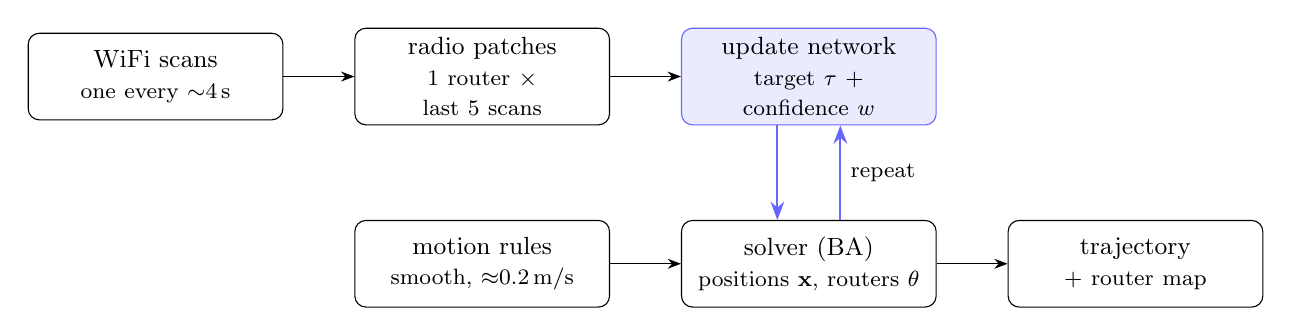
\begin{tikzpicture}[node distance=7mm and 9mm, >=Stealth,
  box/.style={draw, rounded corners, align=center, minimum height=11mm, text width=30mm, font=\small},
  net/.style={box, fill=blue!8, draw=blue!60}]
  \node[box] (scan) {WiFi scans\\ \footnotesize one every $\sim$4\,s};
  \node[box, right=of scan] (patch) {radio patches\\ \footnotesize 1 router $\times$ last 5 scans};
  \node[net, right=of patch] (nn) {update network\\ \footnotesize target $\tau$ + confidence $w$};
  \node[box, below=12mm of nn] (ba) {solver (BA)\\ \footnotesize positions $\x$, routers $\theta$};
  \node[box, left=of ba] (rules) {motion rules\\ \footnotesize smooth, $\approx$0.2\,m/s};
  \node[box, right=of ba] (out) {trajectory\\ \footnotesize + router map};
  \draw[->] (scan) -- (patch); \draw[->] (patch) -- (nn);
  \draw[->] (rules) -- (ba); \draw[->] (ba) -- (out);
  \draw[->, blue!60, thick] ([xshift=-4mm]nn.south) -- ([xshift=-4mm]ba.north);
  \draw[->, blue!60, thick] ([xshift=4mm]ba.north) -- node[right, font=\footnotesize, text=black]{repeat} ([xshift=4mm]nn.south);
\end{tikzpicture}
\end{center}

\section*{2\quad DPVO versus DPRO}
\begin{center}\small
\begin{tabular}{@{}ll@{}}
\toprule
DPVO (camera) & DPRO (WiFi) \\
\midrule
image frame & scan $j$: RSSI $y_{j,a}$ of the routers $a$ heard \\
patch: $3\times3$ pixels in one frame & radio patch $k$: one router $a_k$ over the scans $i_k-4,\dots,i_k$ \\
unknown depth of each patch & unknown router parameters $\theta_a=(\p_a, P_{0,a}, n_a)$, shared by its patches \\
camera projection & propagation model $h(\x,\theta_a)$, Eq.~(1) \\
find the patch in frame $j$ (2D search) & no search: the router ID gives the match; only the value is uncertain \\
network output: 2D flow + weight & network output: RSSI correction $\delta$ (dB) + weight $w$ \\
BA on poses, Schur on depths & BA on 2D positions, Schur on router parameters, + motion rules \\
trained on synthetic TartanAir & trained on synthetic buildings \\
\bottomrule
\end{tabular}
\end{center}

\section*{3\quad Notation and physics model}
Scans $j=1,\dots,N$ at times $t_j$. $H_j$ = routers heard in scan $j$, with RSSI $y_{j,a}$ (dBm).
Unknowns: robot positions $\x_j\in\mathbb{R}^2$ and router parameters $\theta_a=(\p_a\in\mathbb{R}^2,\,P_{0,a},\,n_a)$.
The expected RSSI of router $a$ at position $\x$ (log-distance model):
\begin{equation}
h(\x,\theta_a)=P_{0,a}-10\,n_a\log_{10}\!\big(\lVert \x-\p_a\rVert+\varepsilon\big),\qquad \varepsilon=0.5\ \text{m}.
\end{equation}
$P_{0,a}$ is the router's strength near it; $n_a$ is how fast its signal fades with distance.

\paragraph{Patches and links.} For every scan $i$, $M=6$ heard routers are picked at random; each gives a
patch $k=(i_k,a_k)$. Patch $k$ is linked to every scan $j$ with $|i_k-j|\le R=6$. A link $(k,j)$ asks:
\emph{what RSSI should router $a_k$ have at scan $j$?}

\section*{4\quad The network (one update)}
For each link $(k,j)$ the network reads a feature vector $c_{kj}$:
the measured RSSI of router $a_k$ in scans $j-2,\dots,j+2$ with a heard/not-heard mask;
the model prediction $h(\x_{j'},\theta_{a_k})$ for the same scans and the difference;
how alike scans $i_k$ and $j$ are (mean $|\Delta$RSSI$|$ over shared routers, share of shared routers);
the time gap $t_j-t_{i_k}$; the current distance $\lVert\x_j-\p_{a_k}\rVert$ and $(P_{0,a_k},n_{a_k})$.
A hidden state $z_{kj}\in\mathbb{R}^{64}$ is updated as in DPVO: add the patch context and an MLP of
$c_{kj}$; mix with the same patch's previous and next link; soft-aggregate over links of the same patch,
of the same router, and between the same two scans; two gated residual layers. Two heads give
\begin{equation}
\delta_{kj}=10\cdot f_\delta(z_{kj})\ \text{dB},\qquad w_{kj}=\sigma\!\big(f_w(z_{kj})\big)\in(0,1),\qquad
\tau_{kj}=h(\x_j,\theta_{a_k})+\delta_{kj}.
\end{equation}
$\tau_{kj}$ is the cleaned-up target RSSI, $w_{kj}$ the confidence in it.

\section*{5\quad The solver (bundle adjustment)}
The solver minimises
\begin{align}
\mathcal{E}(\x,\theta)=\;&\sum_{(k,j)} w_{kj}\left(\frac{\tau_{kj}-h(\x_j,\theta_{a_k})}{\sigma}\right)^{\!2}
&&\text{WiFi: match the targets}\nonumber\\
&+\sum_{j}\left\lVert\frac{\x_{j+1}-2\x_j+\x_{j-1}}{\sigma_{\text{acc}}}\right\rVert^2
&&\text{smoothness: no sudden change of step}\nonumber\\
&+\sum_{j}\left(\frac{\lVert\x_{j+1}-\x_j\rVert-v_0\,\Delta t_j}{\sigma_v\,\Delta t_j}\right)^{\!2}
&&\text{speed: fixes the scale}\nonumber\\
&+\sum_a\left[\left(\frac{P_{0,a}-\bar P_0}{\sigma_P}\right)^{\!2}+\left(\frac{n_a-\bar n}{\sigma_n}\right)^{\!2}\right]
&&\text{weak router priors}
\end{align}
with $\sigma=5$\,dB, $\sigma_{\text{acc}}=0.3$\,m, $v_0=0.2$\,m/s, $\sigma_v=0.1$\,m/s, $\bar P_0=-40$\,dBm,
$\sigma_P=15$\,dB, $\bar n=3$, $\sigma_n=1$.

\paragraph{Why the two motion terms.} Without smoothness, the solver bends the path to fit WiFi noise.
Without the speed term, scale is unobservable: multiplying all distances by $s$ only shifts every
$P_{0,a}$ by $10\,n_a\log_{10}s$, so paths shrink.

\paragraph{One Gauss--Newton step.} Linearising gives the normal equations
\begin{equation}
\begin{bmatrix} B & E\\ E^\top & C\end{bmatrix}\begin{bmatrix}\Delta\x\\ \Delta\theta\end{bmatrix}=\begin{bmatrix} v\\ u\end{bmatrix},
\end{equation}
where $C$ is block-diagonal (one $4\times4$ block per router, as DPVO's $1\times1$ block per patch depth).
The routers are eliminated with a Schur complement, then back-substituted:
\begin{equation}
\big(B-EC^{-1}E^\top\big)\Delta\x=v-EC^{-1}u,\qquad \Delta\theta=C^{-1}\big(u-E^\top\Delta\x\big).
\end{equation}
The first 3 positions are fixed (the gauge: they say where the path starts). Only the last 12 positions
move; older ones are frozen. Every step is differentiable, so a loss on the positions trains $\delta$ and $w$.

\section*{6\quad Tracking a run (runtime)}
\begin{algorithm}[h]
\caption{DPRO tracking, one scan at a time}
\begin{algorithmic}[1]
\For{each new scan $j$}
  \State $\x_j \gets \x_{j-1}+\tfrac12\,\tfrac{t_j-t_{j-1}}{t_{j-1}-t_{j-2}}\,(\x_{j-1}-\x_{j-2})$ \Comment{damped constant velocity}
  \State pick $M=6$ heard routers at random $\to$ new patches; initialise any new router $\theta_a$
  \State add links: recent patches $\to$ scan $j$; new patches $\to$ scans $j-6..j$
  \If{$j=8$} repeat 12 times: \textsc{Update} \Comment{start-up}
  \ElsIf{$j>8$} repeat 2 times: \textsc{Update}
    \State links whose patch is older than 20 scans leave the network but stay in the solver
  \EndIf
\EndFor
\State repeat 12 times: \textsc{Update} with every position free \Comment{final refinement}
\Statex
\Procedure{Update}{}
  \State network on every active link $(k,j)$: $\tau_{kj}, w_{kj}$ \Comment{Eq.~(2)}
  \State 2 Gauss--Newton steps on Eq.~(3) over active and retired links
\EndProcedure
\end{algorithmic}
\end{algorithm}

\section*{7\quad Training}
\begin{algorithm}[h]
\caption{One training step (as DPVO's \texttt{train.py})}
\begin{algorithmic}[1]
\State draw a clip of 15 scans from a new synthetic building (true positions $\g_j$, noise-free RSSI known)
\State start with 8 scans, positions all at the last fixed one (DPVO starts at identity)
\For{iteration $s=1,\dots,18$}
  \If{$s>8$} add the next scan (position copied from the previous one) and its links \EndIf
  \State \textsc{Update} (network $+$ 2 solver steps)
  \State $\mathcal{L}_{\text{pose}}^{(s)}=\frac1n\sum_j\lVert R\x_j+\mathbf{t}-\g_j\rVert$ \Comment{$R,\mathbf{t}$: best rigid fit, mirror allowed, not differentiated}
  \State $\mathcal{L}_{\text{rssi}}^{(s)}=\frac{1}{|E|}\sum_{(k,j)}|\tau_{kj}-y^{\text{true}}_{j,a_k}|/\sigma$ \Comment{synthetic only}
\EndFor
\State $\mathcal{L}=\sum_s 0.9^{\,18-s}\big(\mathcal{L}_{\text{pose}}^{(s)}+0.5\,\mathcal{L}_{\text{rssi}}^{(s)}\big)$; AdamW step
\end{algorithmic}
\end{algorithm}
The first 300 clips keep positions fixed to the truth and train only $\mathcal{L}_{\text{rssi}}$
(DPVO does the same for its first 1000 steps). We use 4000 clips, 3 independent trainings.

\paragraph{Synthetic buildings.} A grid of corridors 6--12\,m apart (20\,\% removed); wall lines every
3--8\,m, each costing 3--8\,dB; 12--30 routers with $P_0\in[-42,-28]$\,dBm, $n\in[2,3.2]$ and a fixed
shadowing pattern of 3--7.5\,dB; reading noise 2.5--4.5\,dB; detection threshold $-88$ to $-82$\,dBm;
5--25\,\% random drop-outs; robot at 0.12--0.3\,m/s, one 3.5\,s scan every $\sim$4\,s, each router read at
a random instant of the scan. Ranges tuned so the statistics match the real building.

\section*{8\quad Solvers without the network (baselines)}
Same patches, links and solver; only $\tau$ and $w$ change:
\begin{center}\small
\begin{tabular}{@{}lll@{}}
\toprule
name & target $\tau_{kj}$ & weight $w_{kj}$ \\
\midrule
network off & measured $y_{j,a_k}$ & 1 if heard, 0 if not \\
network off, tuned & measured $y_{j,a_k}$ & 0.1 if heard, 0 if not (0.1 chosen on synthetic data) \\
motion rules only & -- & 0 \\
DPRO & $h+\delta_{kj}$ from the network & $w_{kj}$ from the network \\
\bottomrule
\end{tabular}
\end{center}
Results (mean of per-run median error after rigid alignment, 12 real runs): motion rules only 3.57\,m,
network off 2.70\,m, network off tuned 1.47\,m, DPRO 1.51\,m ($\pm$0.02 over 3 trainings).

\end{document}
